

\section{Background}


% \begin{table}[!t]
% \centering
% \caption{The config of three typical drafters} \label{tab:latency}
% \begin{tabular}{@{}ccccc@{}}
% \toprule
% Architecture & EAGLE-3 (Autoregressive) & DFlash (Parallel) & DSpark (Semi-autoregressive) &  \\ \midrule
% Loss Function & KL divergence & Token-level CE & Token-level CE+TV &  \\ \midrule
% $\texttt{Time}_{M_D}(N)$ & $N \times L \times t$ & $L \times t$ & $L \times t + \gamma$ &  \\ \bottomrule
% \end{tabular}
% \end{table}

\subsection{Speculative Decoding}
% Speculative decoding accelerates LLM inference through a draft-and-verify pipeline. Given the current context, a lightweight draft model ($M_D$) generates $N$ candidate tokens ($\texttt{Time}_{M_D}(N)$), which are then verified in parallel ($\texttt{Time}_{M_T}(N)$) by the target model ($M_T$). The target model accepts a prefix of these candidates based on an acceptance criterion (\textit{e.g.}, rejection sampling) and typically recovers one additional token, totally generating $AL$ ($1 \sim N+1$) tokens by a single forward. Therefore, the practical speedup can be formulated  as follows~\cite{nvidiaspec}.
Speculative decoding accelerates LLM inference through a draft-and-verify pipeline shown in Figure~\ref{fig:background}(a). Given the current context, a lightweight draft model \(M_D\) generates \(N\) candidate tokens, which are subsequently verified in parallel by the target model \(M_T\). If \(\tau\) tokens are produced per verification round, the practical speedup~\cite{nvidiaspec} can be approximately expressed as

\begin{equation}
    \mathrm{Speedup} = \frac{\mathrm{Time}_{M_T}(1) \times \tau}{\mathrm{Time}_{M_T}(N)+\mathrm{Time}_{M_D}(N)}
\end{equation}

Therefore, speculative decoding performance mainly depends on two factors: acceptance length \(\tau\) and draft-model latency \(\mathrm{Time}_{M_D}(N)\).

Existing draft models mainly follow three architectural paradigms, summarized in Figure~\ref{fig:background}(b)(c)(d). Autoregressive drafters, represented by EAGLE~\cite{li2026eagle3}, explicitly preserve causal dependencies among speculative tokens but require sequential draft steps. Parallel drafters, such as DFlash~\cite{chen2026dflash}, predict all speculative positions in one forward pass, substantially reducing drafting latency but removing intra-block causal dependency. Semi-autoregressive drafters, including DSpark~\cite{cheng2026dspark} and Domino~\cite{huang2026domino}, combine a parallel backbone with a lightweight sequential module to balance drafting latency and prediction quality. Despite their different structures, these designs share one property: the draft model still explicitly depends on the historical context, whose length grows with decoding. In contrast, Figure~\ref{fig:background}(e) shows that \we removes this growing historical dependency by directly reusing contextual features produced by the target model and performs local prediction.

% Two important factors, $AL$ and $\texttt{Time}_{M_D}(N)$, depend on the capability and efficiency of the draft model, respectively. Therefore, various studies have explored many techniques to optimize these two factors. These studies can be broadly categorized into three model architecture paradigms, and the latency of these three architectures is formulated in Table~\ref{tab:latency}. The $L$ denotes the number of layers in the draft model, and the $t$ denotes the latency of executing a single transformer layer, and the $\gamma$ denotes the latency of executing the sequential module.

% \subsubsection{Autoregressive Architecture}
% Autoregressive drafters generate speculative tokens sequentially and explicitly model the causal dependency among draft tokens. EAGLE~\cite{li2024eagle,li2024eagle2,li2026eagle3} is the representative of this architecture, which leverages hidden states from the target model and employs a single transformer layer for autoregressive generation. Similar designs have also been introduced into industrial LLMs (\textit{e.g.}, DeepSeek-V4~\cite{xu2026deepseek} and GLM-5.2~\cite{zeng2026glm}) through native multi-token prediction (MTP) modules during post training. 
% The latency of these autoregressive draft models can be formulated as follows.

% \begin{equation}
%     \texttt{Time}_{M_D}(N) \approx N \times L \times t
% \end{equation}
% The $L$ denotes the number of layers in the draft model and the $t$ denotes the latency of executing a single transformer layer.


% \subsubsection{Parallel Architecture}
% To maximize execution efficiency, parallel drafters entirely eliminate the sequential generation dependency. The representative work, DFlash~\cite{chen2026dflash}, generates all $N$ candidate tokens simultaneously in a single forward pass on the current context. This design effectively reduce the latency and highly utilizes GPU parallelism. Therefore, this latency is formulated as follows.

% \begin{equation}
%     \texttt{Time}_{M_D}(N) \approx L \times t
% \end{equation}


% \subsubsection{Semi-autoregressive Architecture}
% Semi-autoregressive drafters aim to combine the advantages of the above two paradigms. DSpark~\cite{cheng2026dspark} and Domino~\cite{huang2026domino} employ a parallel backbone to efficiently model the speculative block like DFlash and introduce a lightweight sequential module to capture dependencies among draft tokens. In this way, the computationally expensive contextual modeling remains parallel, while only a lightweight component is executed sequentially. Such designs provide a better trade-off between acceptance quality and drafting latency, making semi-autoregressive drafting particularly attractive for practical serving systems. 

\begin{figure}[!t]
    \centering
    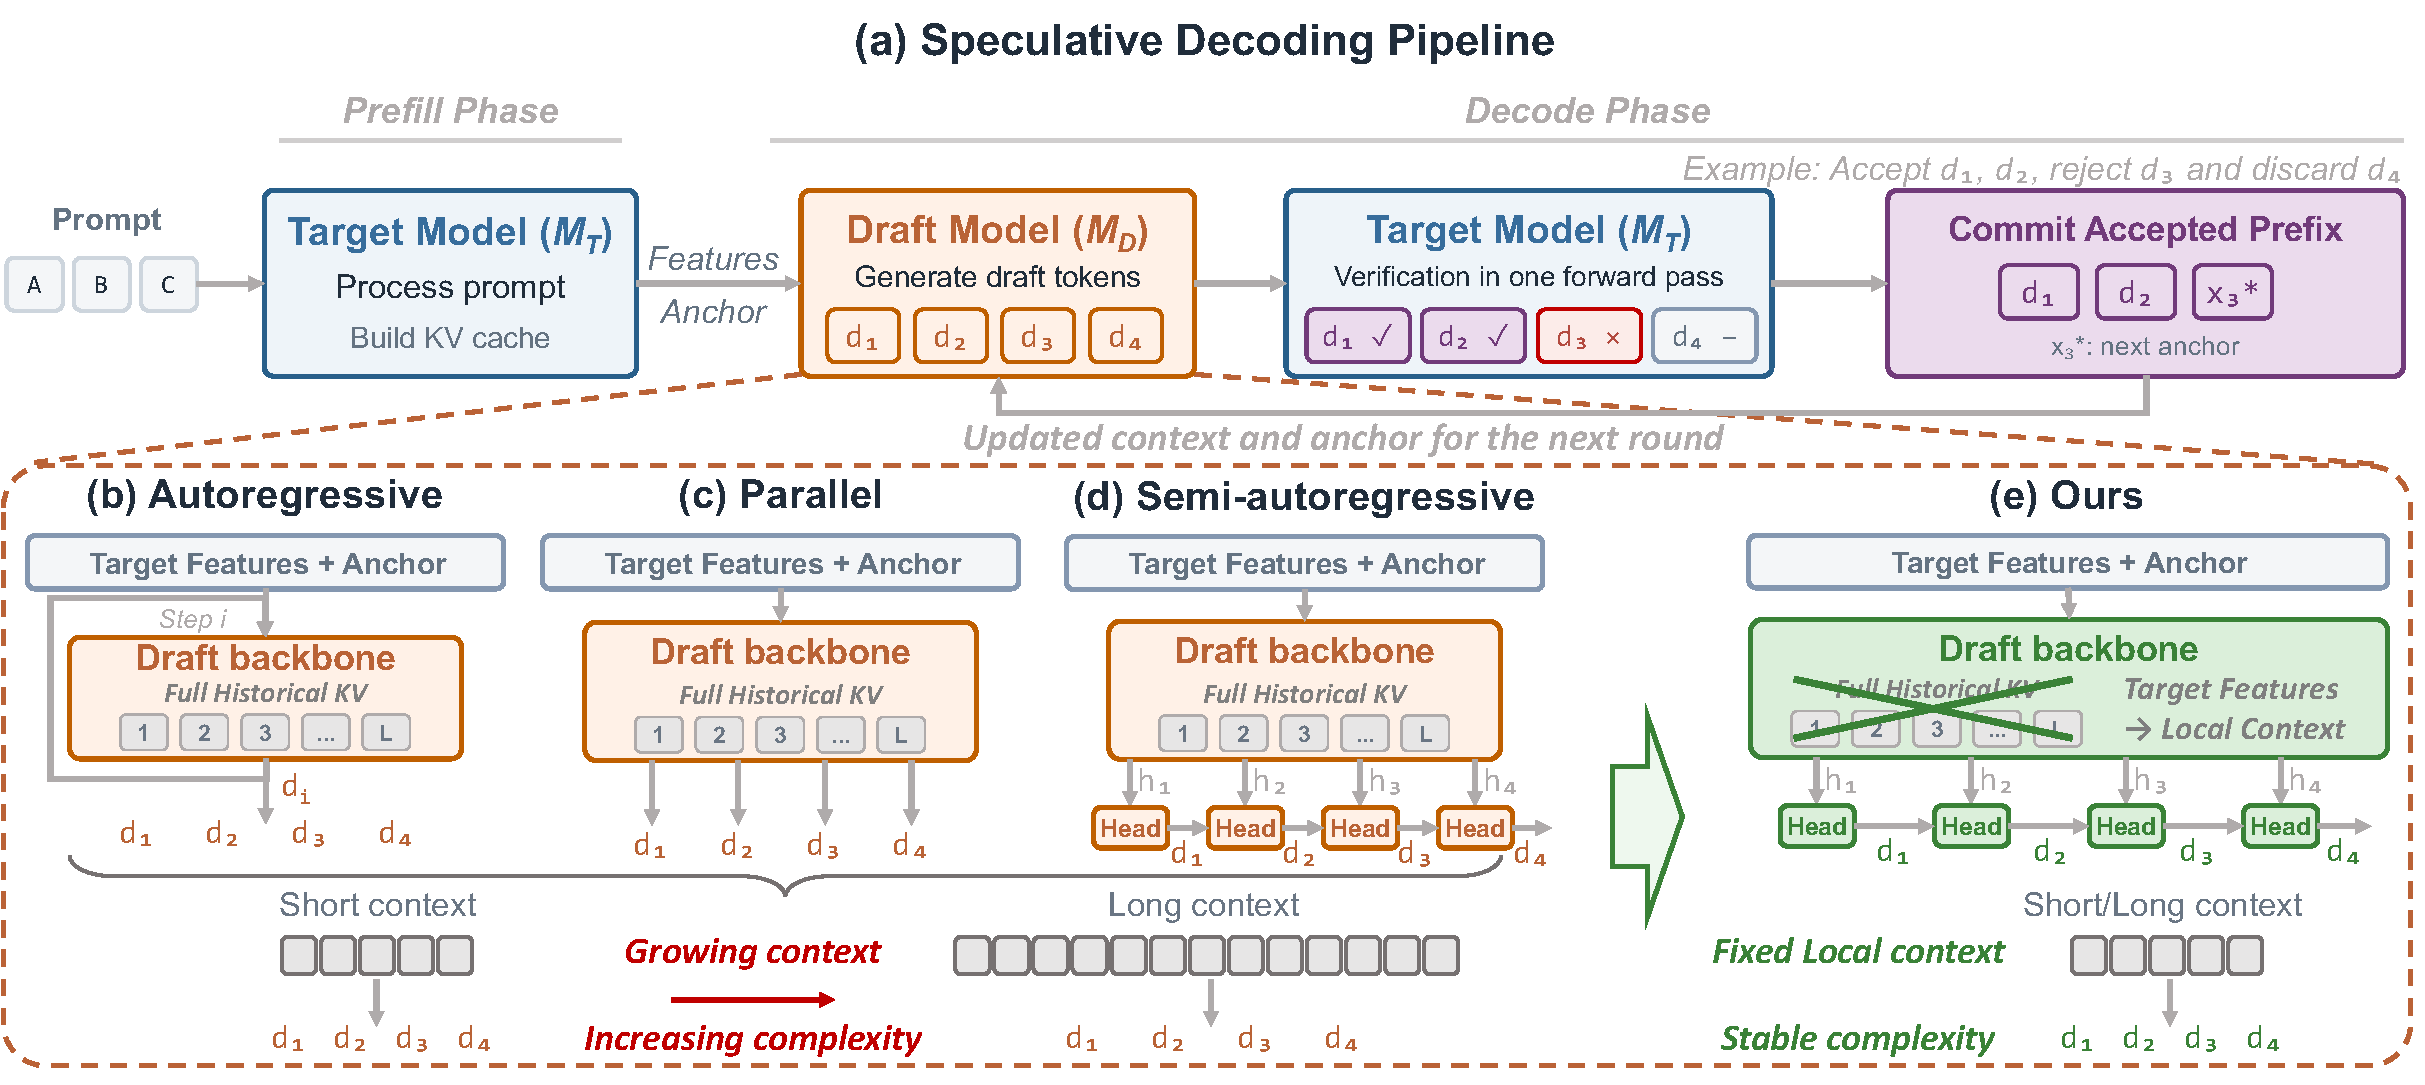
\includegraphics[width=0.98\textwidth]{fig/background2.pdf}
    % \vspace{-10pt}
    \caption{Speculative decoding pipeline and comparison of existing draft architectures with \we.}
    \label{fig:background}
    \vspace{-15pt}
\end{figure}



\subsection{Model Distillation}

Training a speculative draft model can be viewed as knowledge distillation from the target model. Different architectures adopt different supervision objectives. EAGLE performs distribution-level distillation using soft-target cross-entropy (CE), which is equivalent to minimizing forward Kullback-Leibler divergence up to a constant. DFlash primarily adopts token-level CE, while DSpark combines CE with total variation (TV) distance to improve distribution overlap between the draft and target models. Domino applies token-level supervision to both parallel and causally corrected predictions through a training curriculum. These differences are particularly relevant to \we because its history-free prediction structure differs substantially from the autoregressive target model, making direct distribution-level distillation non-trivial.

% The training of speculative draft models can be naturally viewed as knowledge distillation from the target model, while different drafting architectures adopt different supervision objectives. EAGLE~\cite{li2026eagle3} performs distribution-level distillation using soft-target cross-entropy ($\mathcal L_{\mathrm{cls}}=-\sum_v p_t(v)\log p_d(v)$), which is equivalent to minimizing the forward Kullback-Leibler divergence between the target and draft distributions up to the constant entropy of the target distribution. In contrast, DFlash~\cite{chen2026dflash} primarily trains its parallel draft model using position-weighted token-level cross-entropy ($\mathcal L_{\mathrm{CE}}=-\sum_k w_k \log q_k(x_k)$), while DSpark~\cite{cheng2026dspark} further combines cross-entropy with total variation (TV) distance ($\mathcal L_{\mathrm{TV}}=\sum_k w_k\|p_k^d-p_k^t\|_1$) to directly improve the distribution overlap that determines speculative acceptance. Domino~\cite{huang2026domino} jointly applies token-level cross-entropy to the parallel backbone and the causally corrected predictions with a training curriculum that gradually shifts optimization toward the latter. 

% Although forward KL is widely adopted in conventional knowledge distillation, directly applying distribution-level distillation becomes less natural for parallel and semi-autoregressive drafters because their prediction structures and conditioning information are different from those of the autoregressive target model. The difficulty is therefore not that heterogeneous architectures mathematically prevent KL-based distillation, but that the target and draft distributions are produced under different conditioning structures, making direct distribution alignment less effective. Consequently, these methods typically rely more heavily on token-level supervision and introduce architecture- or acceptance-aware objectives to train their draft models.






\section{Motivation} \label{sec:motivation}

\subsection{Two Important Observations}

Agentic workloads expose two limitations of existing speculative decoding methods: degraded acceptance length and increasing historical-state maintenance overhead.

% As illustrated in Figure~\ref{fig:agent}(a), agents introduce workload characteristics substantially different from conventional conversational inference. With the orchestration of agent harness framework, a single task typically consists of frequent multi-turn LLM interactions with heterogeneous context compositions and execution trajectories. Each turn is often characterized by a long input and a short output, while the accumulated context continuously grows across turns. We find that these workload characteristics expose two major limitations of existing speculative decoding methods.

\textbf{Degraded Acceptance Length.} As illustrated in Figure~\ref{fig:agent}(b), existing speculative decoding methods achieve high acceptance lengths on general workloads such as GSM8K and MBPP, but degrade substantially on agentic workloads such as SWE-Bench and AgentLongBench. As the context grows, lightweight draft models increasingly struggle to capture the information required to match the target model's predictions, causing acceptance lengths to drop to only \(1\sim2\) tokens in some workloads.

% State-of-the-art speculative decoding (\textit{e.g.}, EAGLE~\cite{li2024eagle}, DFlash~\cite{chen2026dflash}, DSpark~\cite{cheng2026dspark}) methods achieve high acceptance lengths on conventional general benchmarks (\textit{e.g.,} GSM8K and MBPP), but their performance degrades significantly under agentic workloads (\textit{e.g.}, SWE-Bench and Agent LongBench). We point out that, as the context grows, lightweight draft models increasingly struggle to capture the information required for accurate prediction, causing their output distributions to deviate from the target model. Figure~\ref{fig:agent}(b) shows that methods that achieve high acceptance lengths on general workloads drop to only $1\sim2$ accepted tokens on agentic workloads with over 80\% performance loss.

\textbf{KV Cache Maintenance.} Existing speculative drafters must maintain historical KV states for subsequent generation. After each target-model verification, accepted tokens are committed to the draft model to update its KV cache, while prefix caching further requires historical draft states to be preserved across agent turns. Under frequent multi-turn workloads with continuously growing contexts, these operations become increasingly expensive. Using SGLang to evaluate the multi-token prediction module in DeepSeek-V4, we observe that the KV cache  updating and maintenance can account for \(10\%\sim20\%\) of end-to-end inference latency.

% As illustrated in Figure~\ref{fig:background}(a), after the verification in target-model, accepted tokens must be committed to the draft model to update its KV cache to maintain the consistency for subsequent draft generation. Under agentic workloads, frequent short generations and continuously growing contexts make such updates particularly expensive. Moreover, supporting prefix caching across multiple agent turns requires the draft model to retain and manage its own historical KV cache regardless of full attention and sliding window attention. We use SGLang~\cite{zheng2024sglang} to evaluate the overhead of the multi-token prediction module in DeepSeek-V4, and find that the updating and maintenance operations can account for $10\%\sim30\%$ of end-to-end inference latency, significantly reducing the system-level benefit of speculative decoding.


\subsection{Analysis and Findings}

% Although the above limitations manifest differently at the model and system levels, our analysis reveals a common root cause: the \emph{growing historical context}. From the model perspective, existing draft models attempt to independently encode an increasingly long history with only a small fraction of the target model's parameters. The resulting gap in long-context modeling capability leads to progressively less accurate draft predictions and lower acceptance lengths. From the system perspective, preserving the same history requires maintaining an ever-growing KV cache for the draft model, which must be repeatedly updated and managed throughout multi-round agent execution.

% These observations expose a fundamental inefficiency in existing speculative decoding: the lightweight draft model is required to both \emph{understand} and \emph{maintain} the complete historical context, even though the target model has already processed the same context and encoded it into its internal representations. This motivates a different design principle for Agentic workloads: rather than independently reconstructing historical information within the draft model, the drafter should directly exploit the contextual representations produced by the target model and operate without maintaining its own historical context cache.

% Based on this insight, we design \we as a \emph{history-free} speculative decoding framework that removes the draft model's dependence on historical KV cache while preserving the contextual information required for accurate speculation.

Although the above problems appear at different levels, they share a common cause: the draft model is required to independently process and maintain the growing historical context shown in Figure~\ref{fig:background}. From the model perspective, a lightweight drafter has only a fraction of the target model's capacity, making it increasingly difficult to reproduce the target model's long-context representation as history grows. From the system perspective, preserving the same history requires maintaining and repeatedly updating an increasingly large draft KV cache.

The key inefficiency is therefore that the draft model repeatedly reconstructs historical information that has already been processed by the target model. We instead argue that the drafter should directly reuse the target model's contextual representations and dedicate its limited capacity to modeling the information required for local speculative prediction. 
% This observation motivates \we, which removes the draft model's dependence on historical KV cache by directly reusing target hidden states for contextual information and performing only local speculative prediction shown in Figure~\ref{fig:background}(e).
